\subsection{Layer deduplication}
\label{sec:dedup-desgin}

%We now describe \sysname's layer restoring performance--aware deduplication 
% (i.e., \sysname's~\dedupname) system design. 
%\subsubsection{When to deduplicate layers?}
%
%
%\subsubsection{Layer deduplication and partition}

As with the traditional Docker registry, 
\sysname maintains a \emph{layer index}.
After receiving a \texttt{PUT} layer request,
\sysname first checks the \textbf{layer fingerprint} in the \emph{layer index} to ensure 
an identical layer is not already stored.
The layer fingerprint is calculated by hashing the layer content, which is also used as layer identifier denoted as \textbf{layer id}.
After that, \sysname~replicates $r$ primary layer replicas on P-servers. 
Meanwhile, \sysname~submits $R-r$ backup layer replicas to D-servers and temporally stored on layer stage areas.
 % and acknowledges back to the client. 
 After D-servers receive the backup replicas,
 \sysname will first update \emph{RLmap} with the layer and its associated repository, where
RLmap maps a \textbf{repository id} (i.e., repository name) to its containing layers 
as shown in Figure~\ref{fig:dedup-partition}.

%After the layer is deduplicated, it will be removed from stage area.
%\dedupname system~initiates layer deduplication process only if 
%layer deduplication will achieve significant space savings and 
%the process won't impact foreground requests. 
%Sepcially, layer deduplication process is triggered when
%the layer dataset $S$ is greater than a predefined threshold $\theta_{s}$ and 
%the registry traffic $RPS$ ( i.e., requests per second) is lower than $\theta_{RPS}$. Thus, layer deduplication process runs periodically.
%The process always stars with the cold layers that haven't been
%access for a long time.
 
 \sysname initiates a lightweight layer deduplication process which collaborates with the metadata database
 to remove redundant files from layers. 
The deduplication process has three major steps: 
layer decompression, 
file-level deduplication,
\textbf{unique file replication} and \textbf{layer partitioning}. 
The first two steps are necessary for removing duplicate files from compressed layer tarballs.
%<<<<<<< HEAD
The last step -- unique file replication and layer partitioning is 
to evenly distribute the I/O and computation load of layer restoring across D-servers 
while maintain a certain level of fault-tolerance.  
Note that only one layer replica is selected from $R-r$ backup replicas to do layer deduplication.
After the layer replica is \emph{deduplicated}, all the backup layer replicas stored on D-servers will be discarded.  
%=======
%The last two step -- file replication and layer partitioning is 
%to evenly distribute the I/O and computation load of layer restoring across multiple registry servers 
%while also maintaining a level of redundancy.  
%Note that only one layer replica is selected among $R-r$ layer replicas to do layer deduplication. % subil: NEED CLARIFICATION ON WHAT THIS MEANS
%After that, all the layer replicas will be discarded.  
%>>>>>>> ab86d0a4767bfcfcbb58baf9bd7b2e81e54d7e51
%This makes the process of layer restoring achieve the maximum parallelism for each layer to accelerate the restoring process. 
%(detailed in~\cref{subsubsec:slice-restoring}) 
%After layer deduplication, unique files are evenly distributed across multiple registry servers. 

%\begin{figure*}[t]
%		\begin{minipage}{0.21\linewidth}
%			\centering
%			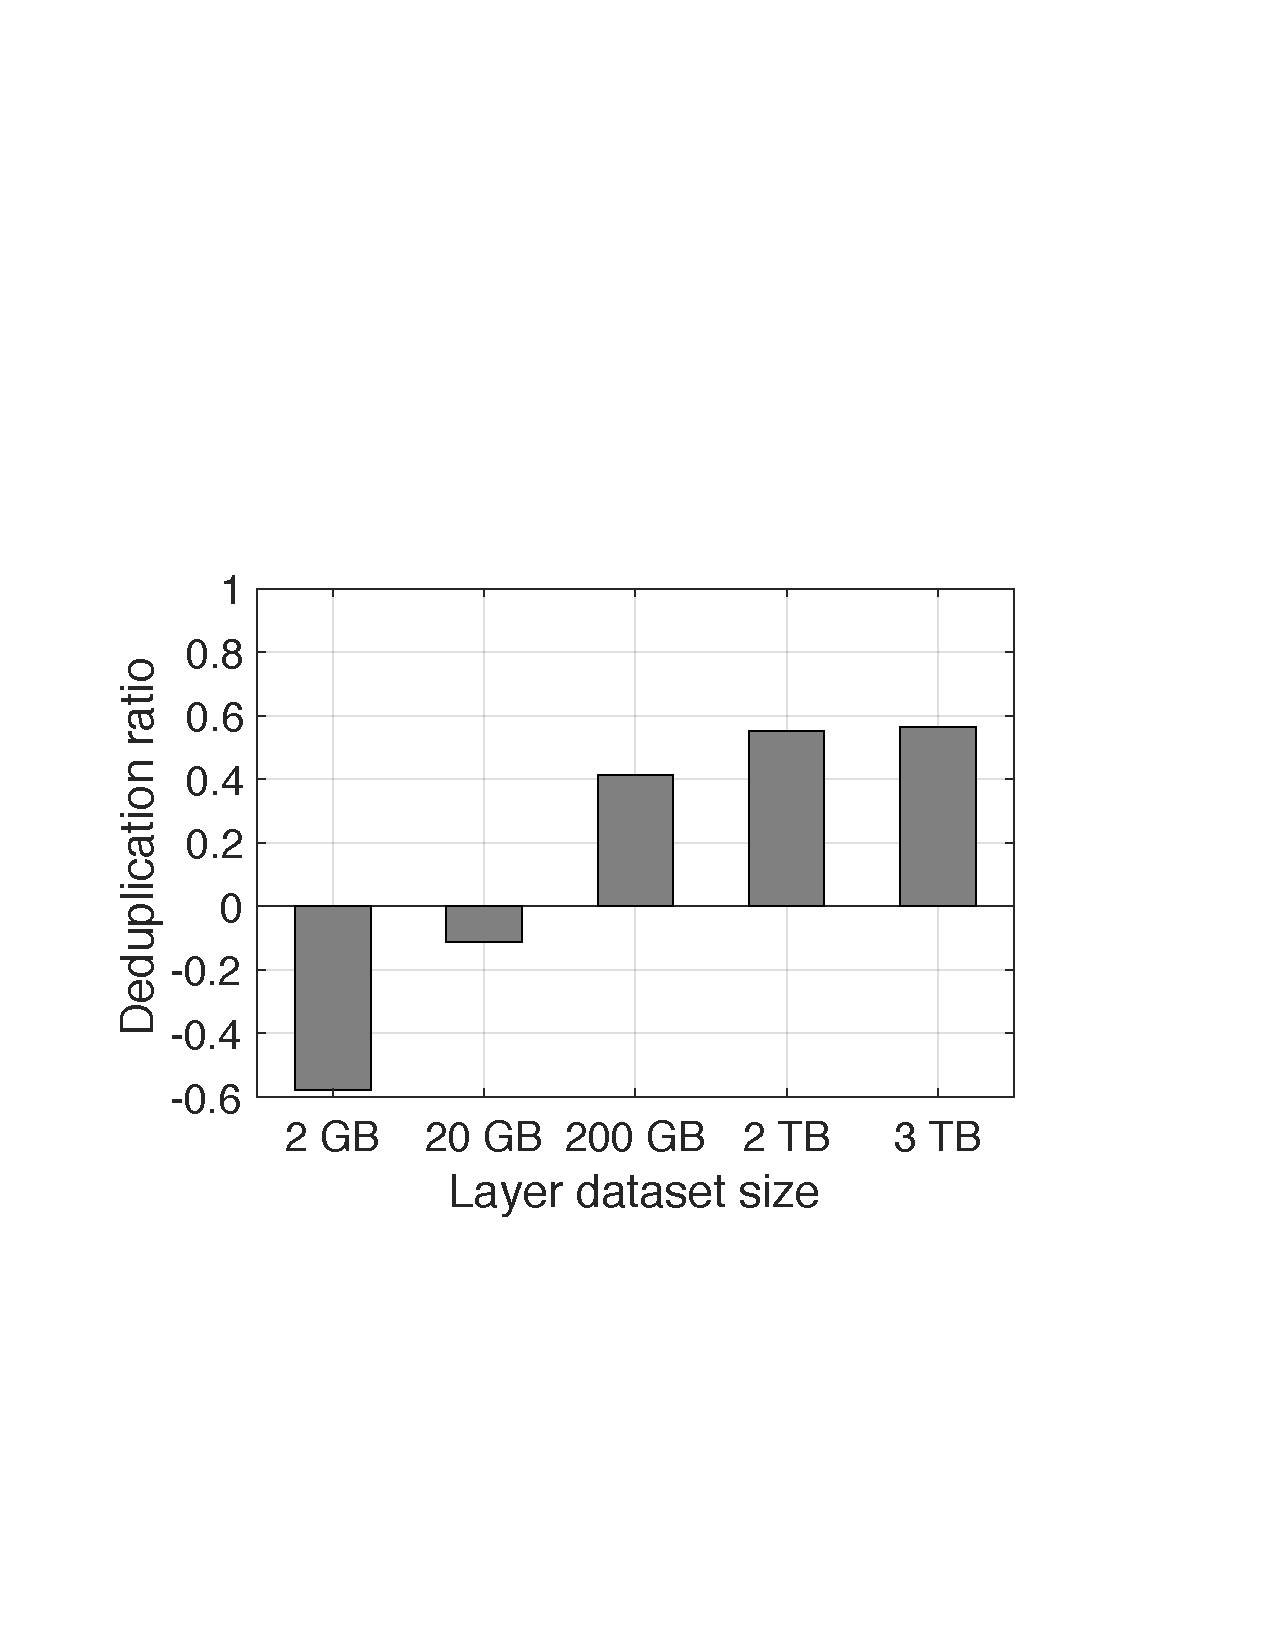
\includegraphics[width=1\textwidth]{graphs/dedup_vs_compression.pdf}
%			\caption{File-level deduplication vs. compression efficiency.}
%		%	\vspace{-3pt}
%			\label{fig:cacheefficiency}
%		\end{minipage}
%			\begin{minipage}{0.38\linewidth}
%				\centering
%				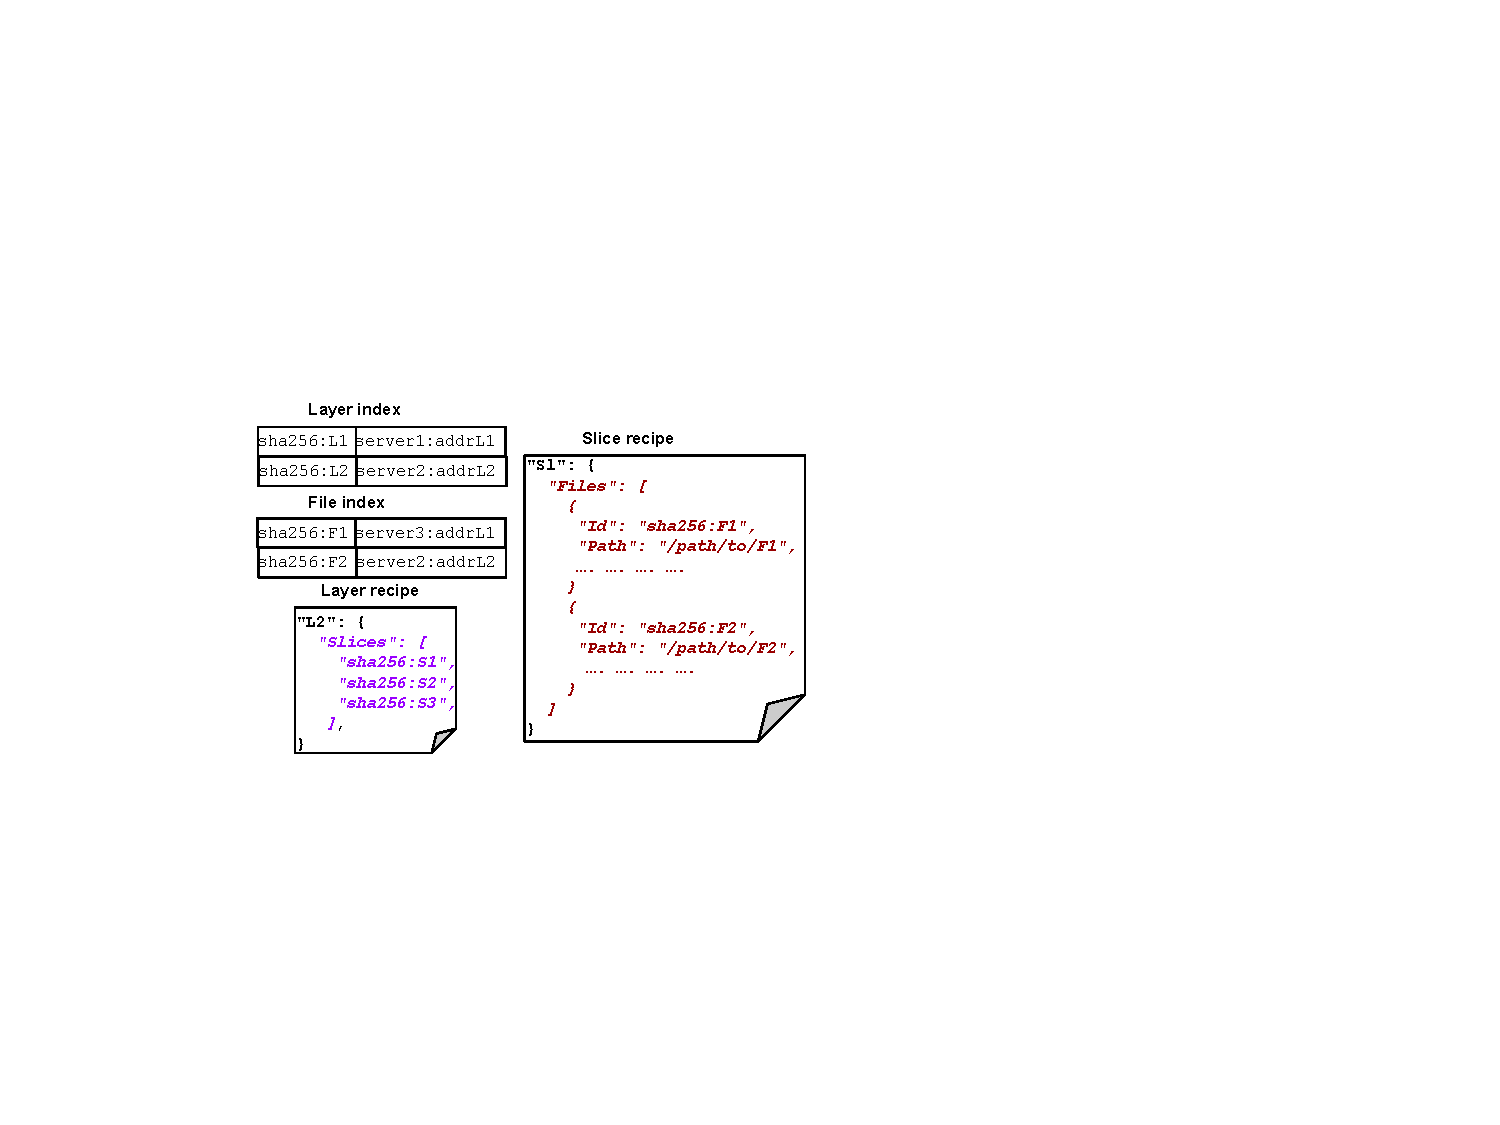
\includegraphics[width=1\textwidth]{graphs/sift-metadata.pdf}
%				\caption{Metadata for deduplication.}
%				%	\vspace{-3pt}
%				\label{fig:sift-metadata}
%			\end{minipage}
%		\begin{minipage}{0.38\linewidth}
%			\centering
%			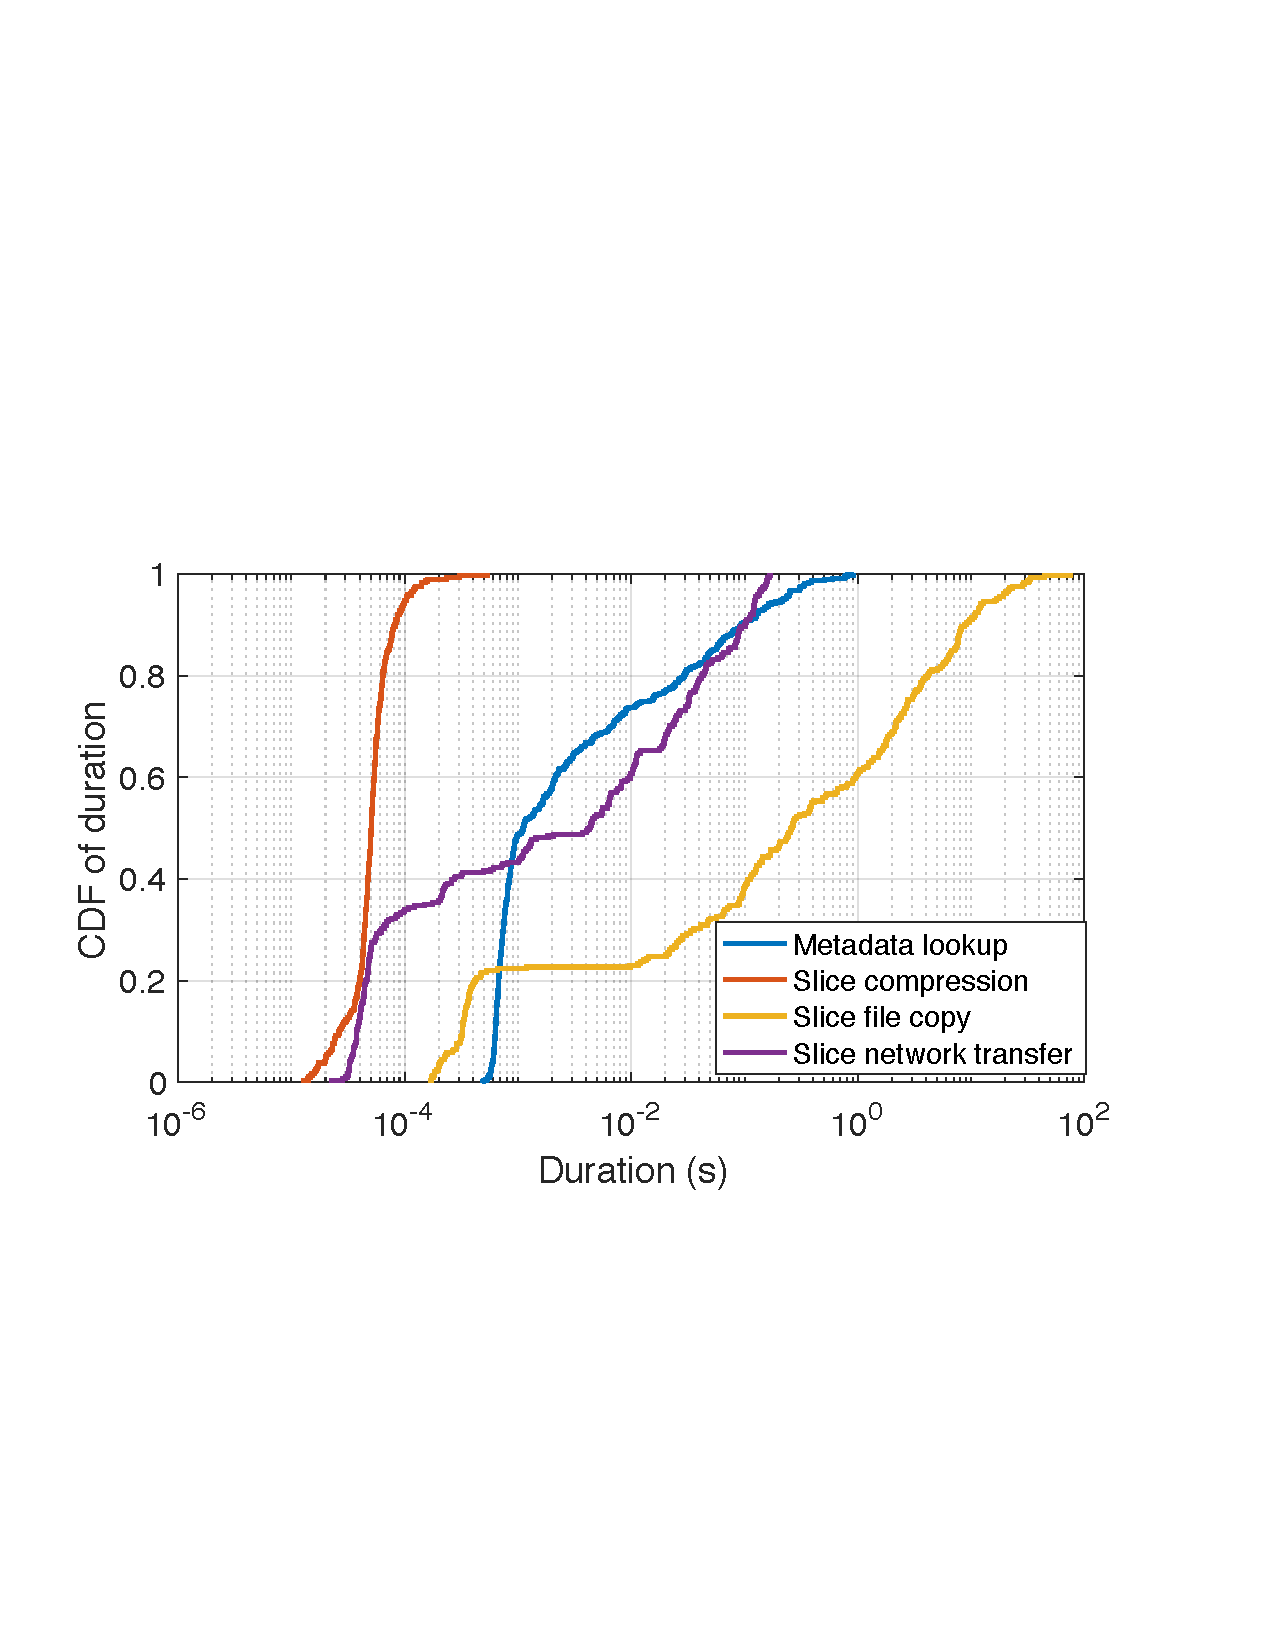
\includegraphics[width=1\textwidth]{graphs/restoring-breakdowns.pdf}
%			\caption{Breakdown of slice restoring time.}
%			%	\vspace{-3pt}
%			\label{fig:slice-restoring-breakdown}
%		\end{minipage}
%\end{figure*}

\begin{figure}[t]
	\centering
	\centering
	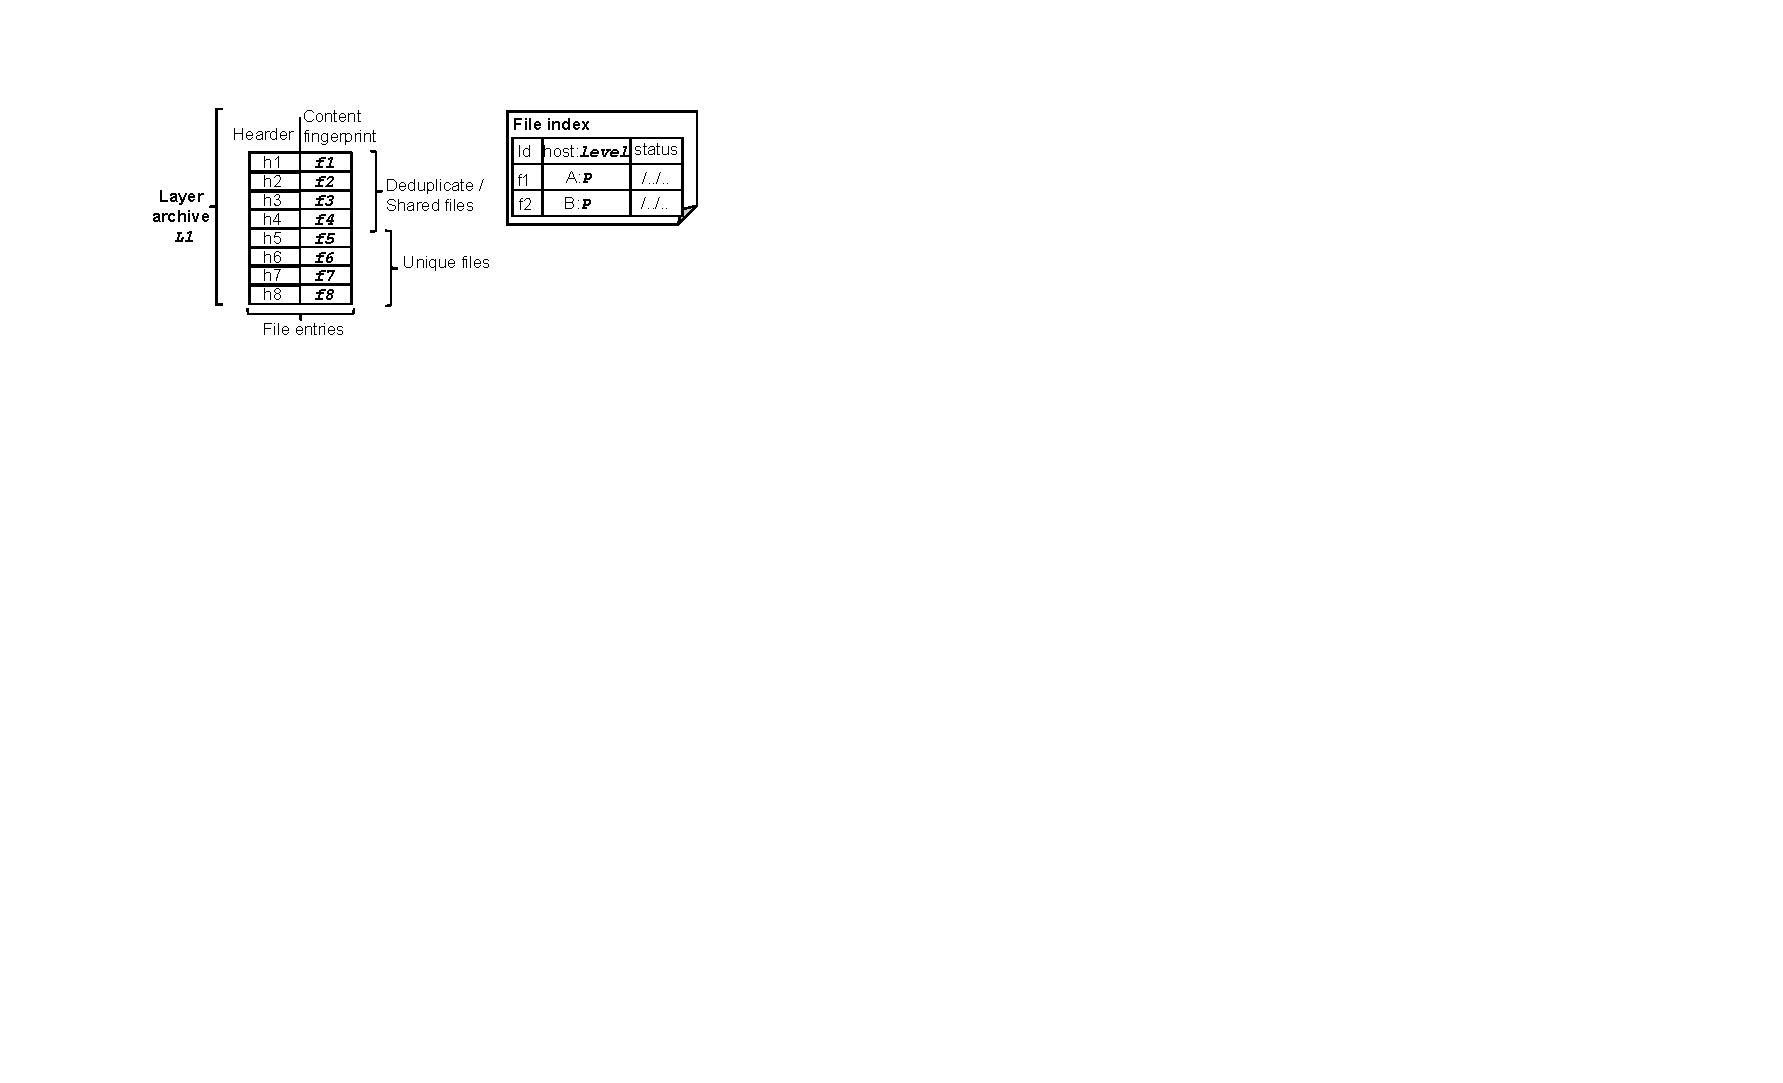
\includegraphics[width=0.45\textwidth]{graphs/sys-architecture-put-layer.pdf}
	\caption{Layer deduplication. \LR{Typo: ``Hearder'' should be ``Header''}}
	\label{fig:dedup-partition}
\end{figure}



%\begin{figure}[t]
%	\centering
%	\begin{minipage}{0.26\textwidth}
%		\centering
%		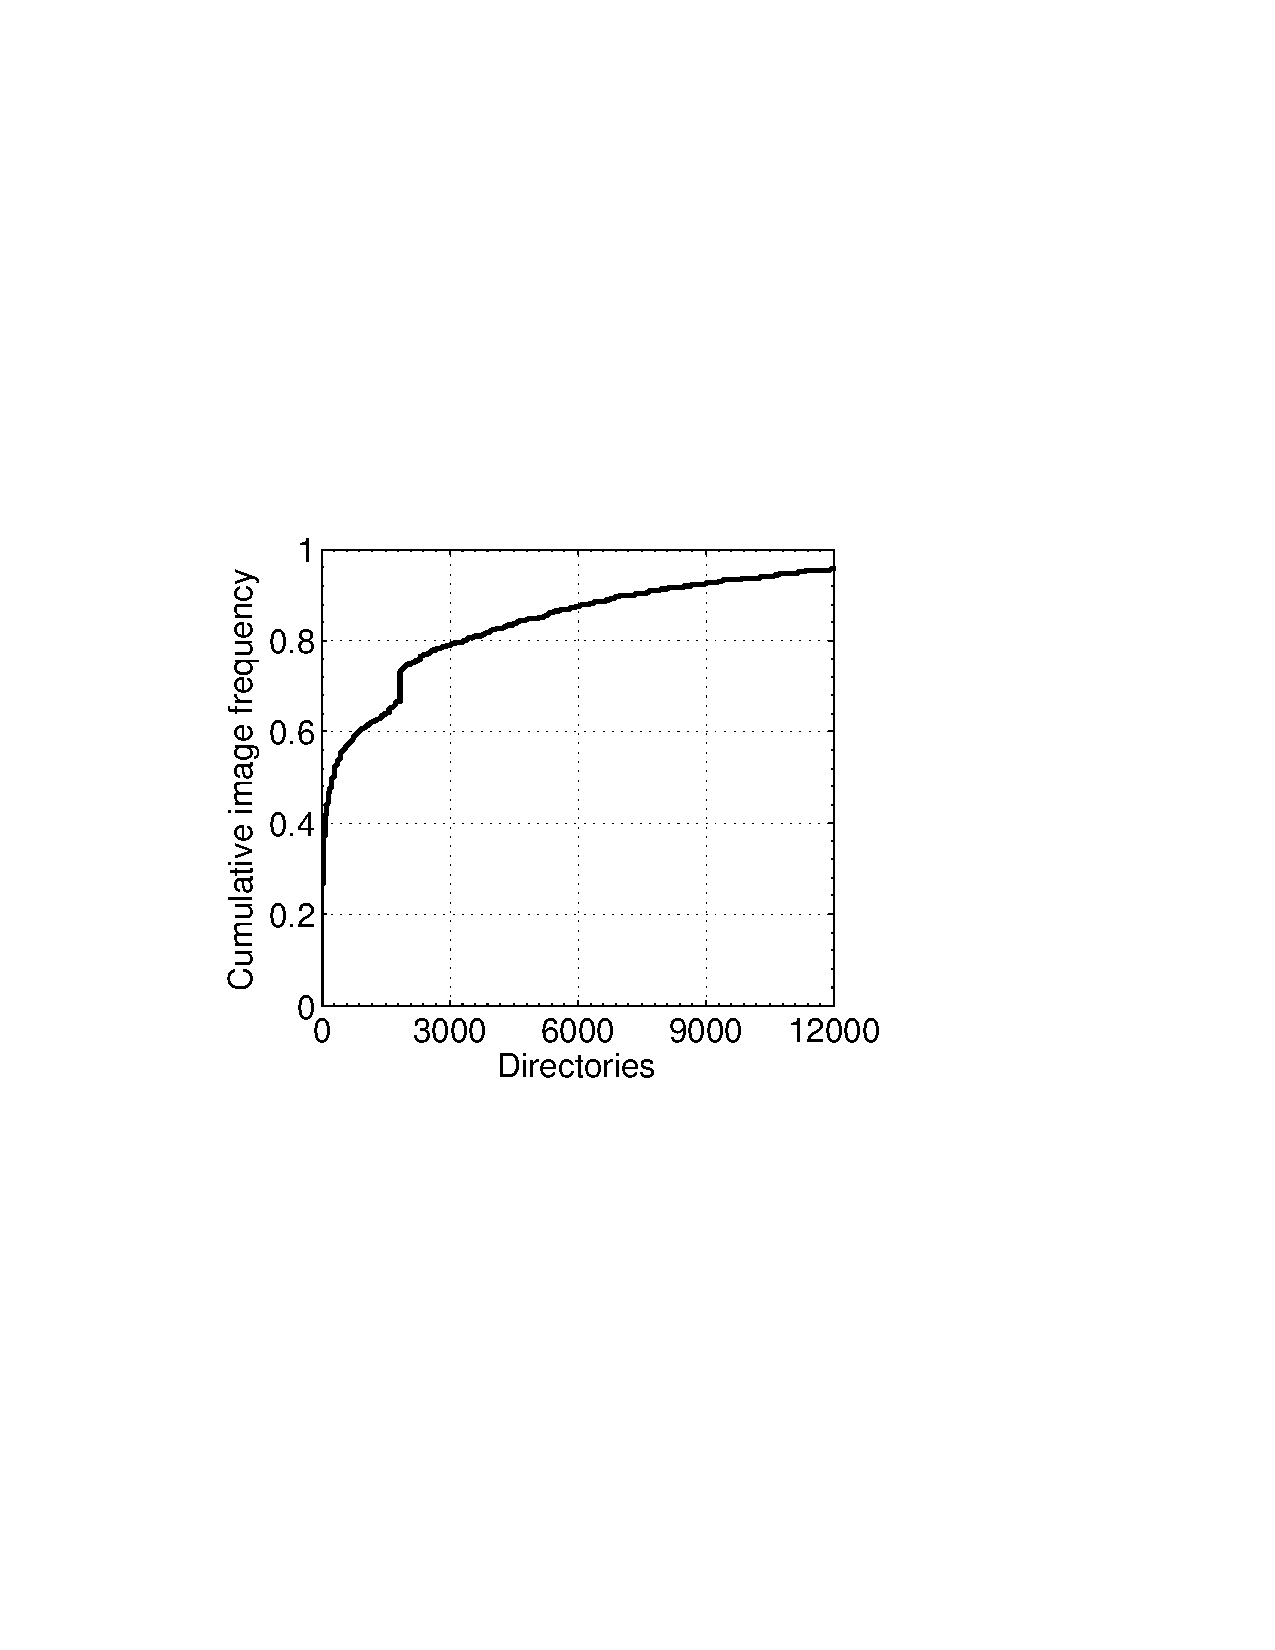
\includegraphics[width=1\textwidth]{graphs/dir.pdf}
%		\caption{CDF of images by\newline directories}
%		\label{fig-dir}
%	\end{minipage}%
%	\begin{minipage}{0.24\textwidth}
%		\centering
%		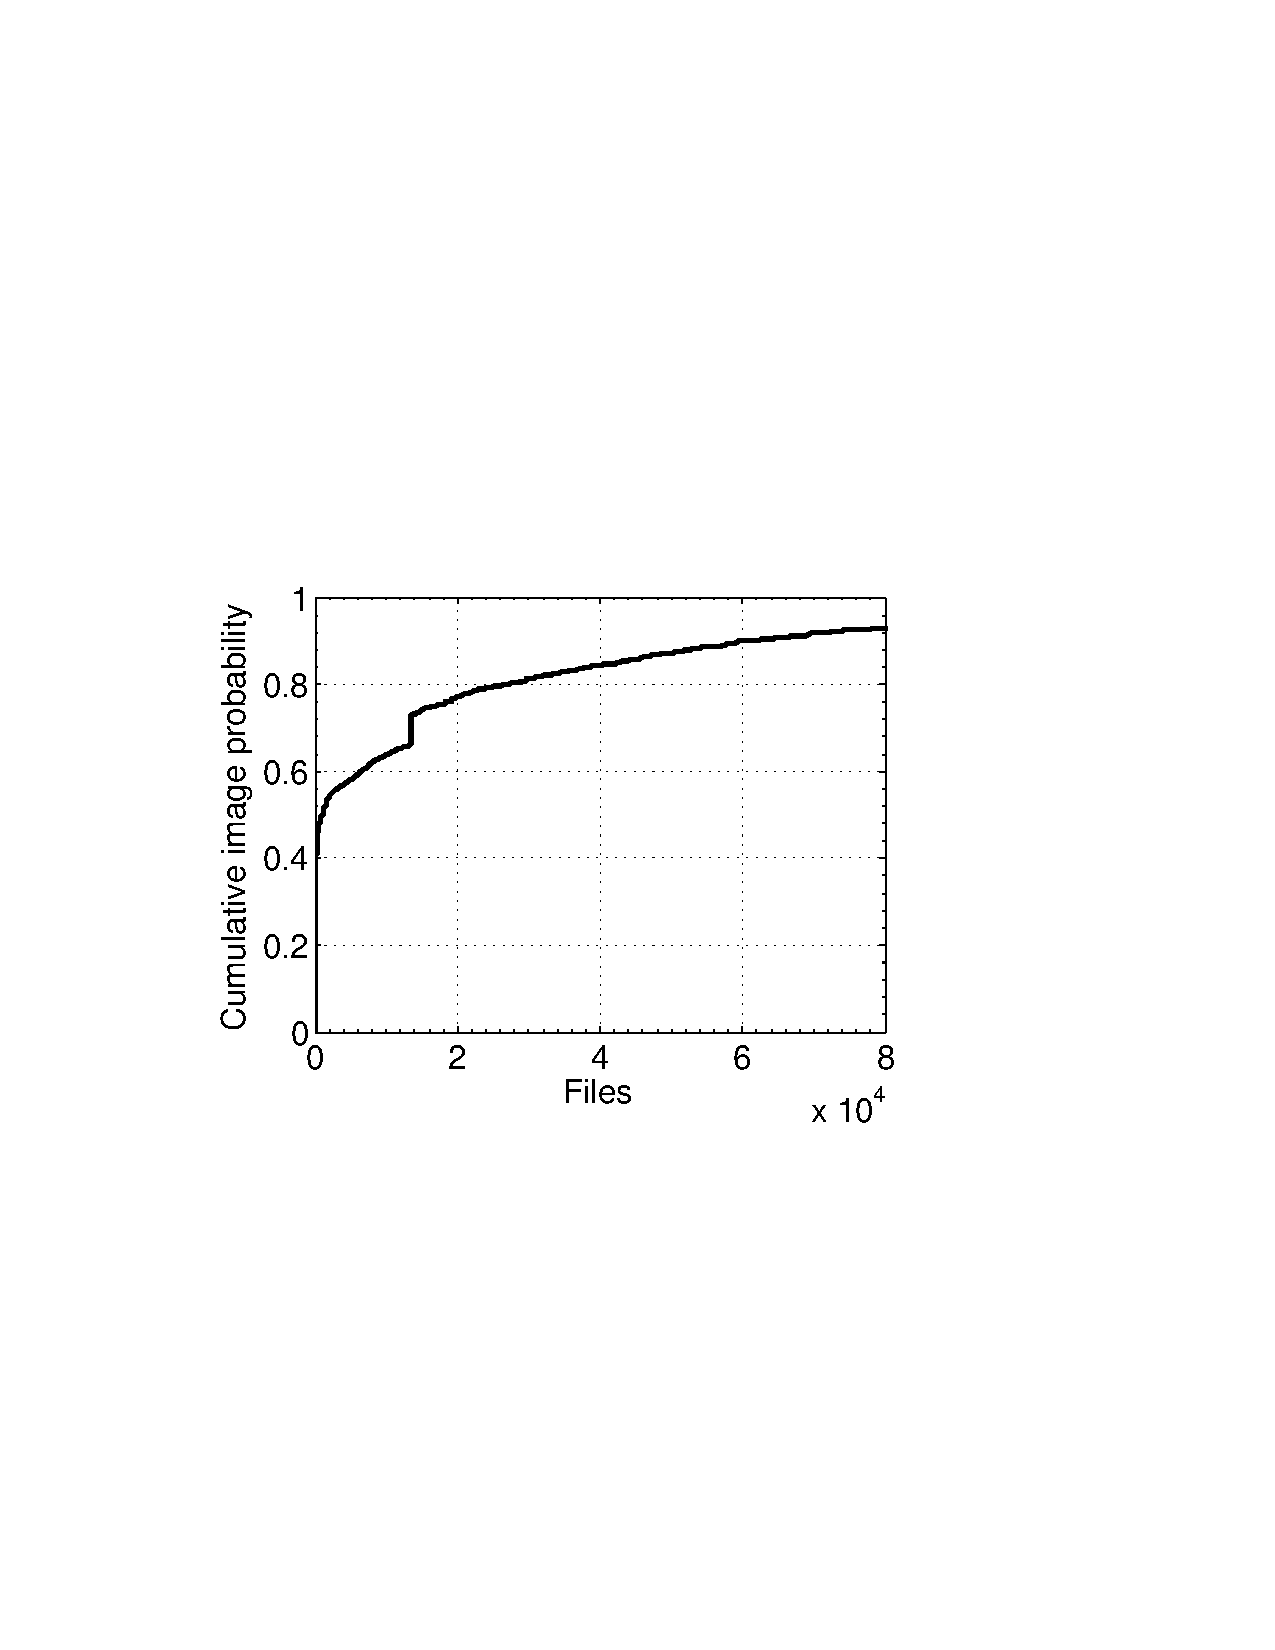
\includegraphics[width=1\textwidth]{graphs/file.pdf}
%		\caption{CDF of images by files}
%		\label{fig-file}
%	\end{minipage}
%\end{figure}

%\begin{figure}[htbp] 
%	\begin{minipage}{0.5\linewidth} 
%		\centering 
%		\includegraphics{circle} 
%		\caption{A Circle} 
%		\label{fig:circle} 
%	\end{minipage}% 
%	\begin{minipage}{0.5\linewidth} 
%		\centering 
%		\includegraphics{rectangle} 
%		\caption{A Rectangle} 
%		\label{fig:rectangle} 
%	\end{minipage} 
%\end{figure}

%\begin{figure}[t]
	\centering
%		\begin{minipage}{0.23\textwidth}
%			\centering
%			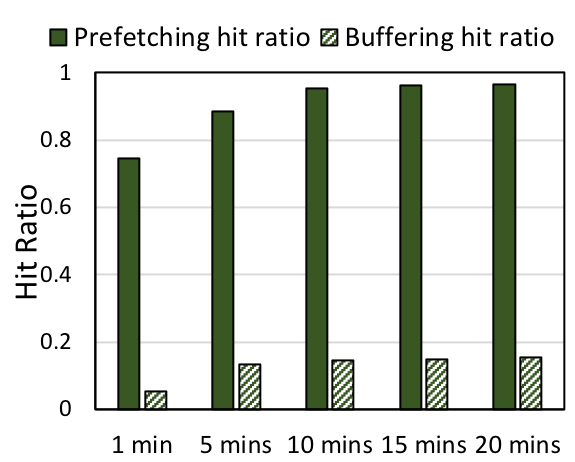
\includegraphics[width=1\textwidth]{graphs/evaluation_hitratios.png}
%			\caption{Hit ratio.}
%			\label{fig:hitratio}
%		\end{minipage}
	%	\begin{minipage}{0.25\textwidth}
			\centering
			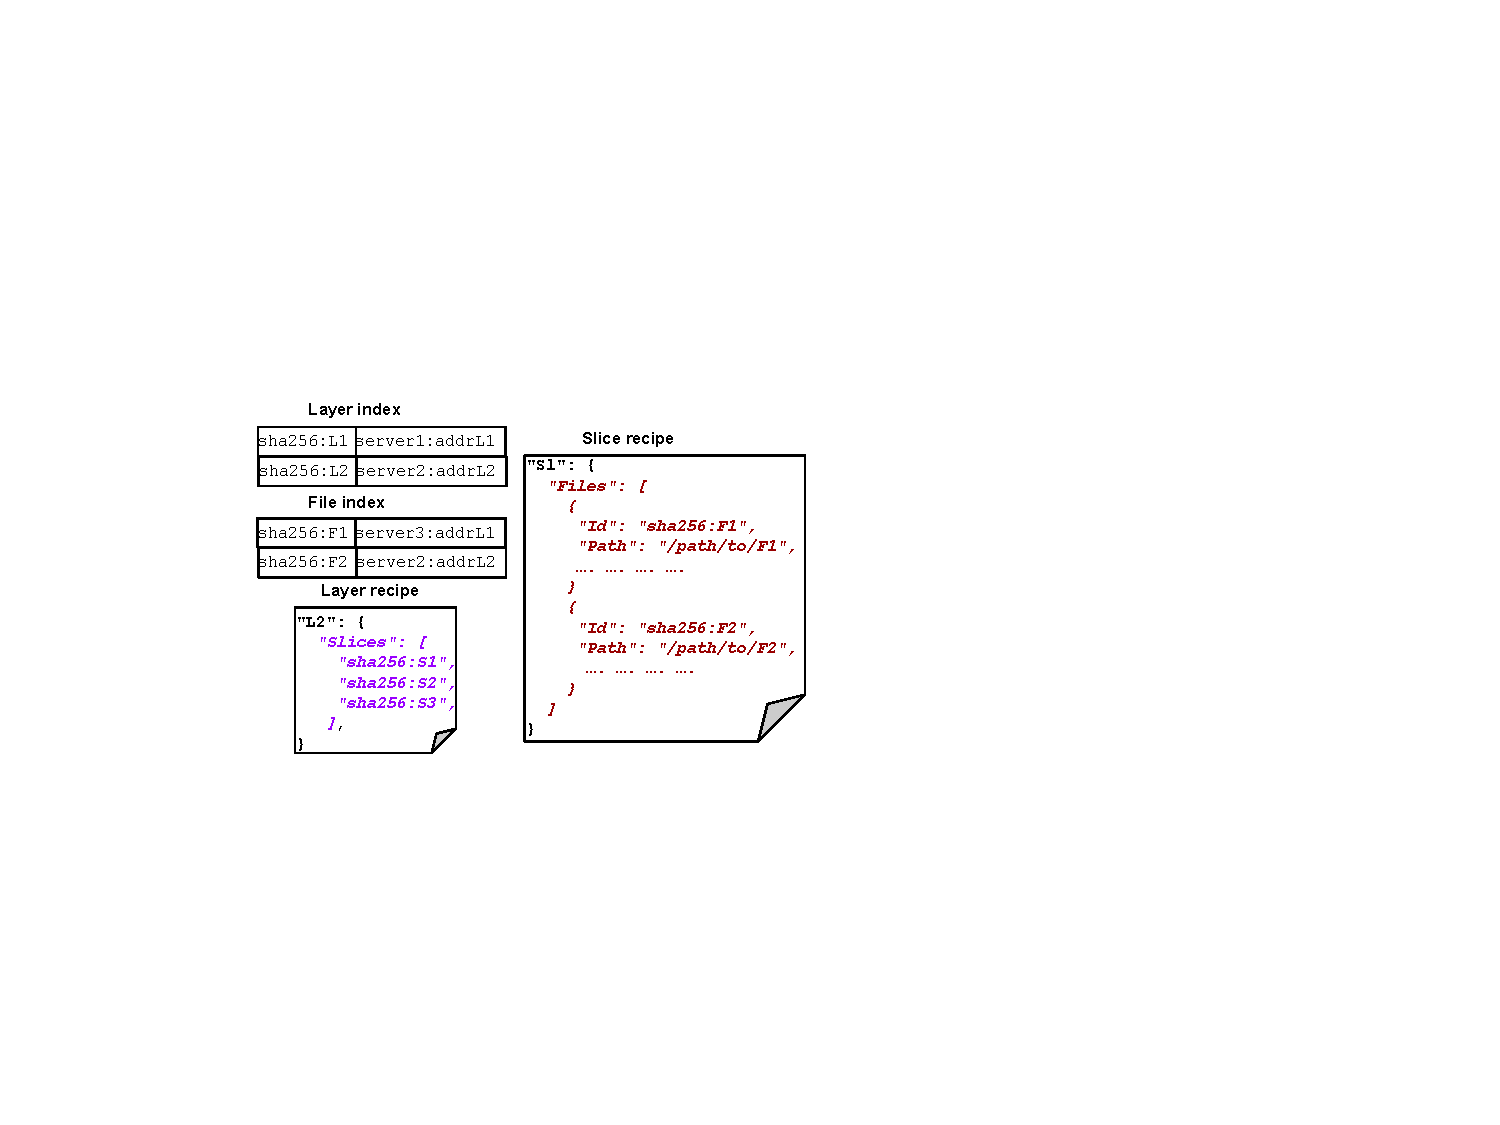
\includegraphics[width=0.4\textwidth]{graphs/sift-metadata.pdf}
			\caption{Metadata for deduplication.}
			%\vspace{-3pt}
			\label{fig:sift-metadata}
	%	\end{minipage}
\end{figure}
\paragraph{Layer file-level deduplication}
As shown in Figure~\ref{fig:dedup-partition}, 
%<<<<<<< HEAD
%a layer is loaded to layer deduplication process.
%First, the layer is decompressed and unpacked into files.
%Next, 
%the process computes a \emph{fingerprint} for every file denoted as \textbf{file id}, 
%and checks every file's fingerprint in the file index.
%If the file is already stored, it will be discard. 
%Otherwise, it will be kept in file store.
%Meanwhile,
%\sysname  records the newly added \emph{file id} to file index.
%\paragraph{Layer partition}
following the staging area, the layer tarball is loaded to the layer deduplication process.
In this process, the layer tarball is first decompressed into a \textbf{layer archive file}.
%Algorithm~\ref{alg:dedup-partition} details layer deduplication and partitioning. 
%After layer decompression, 
Each file entry in the layer archive is represented as a \textbf{file header} and the associated \textbf{file content}.
The file header contains the file name, path, size, mode, owner information, etc.
The file header is needed to rebuild the \emph{file header} for 
the associated file entry in the layer archive.
Thus, 
the process records each file header for every \emph{deduplicated} layers. 
After that,
the process computes a \emph{fingerprint} by hashing the file content denoted as \textbf{file Id}, 
and checks the file Id for presence in the file index.
If the file Id is already stored, the file content will be discarded. 
Otherwise, it will be saved physically in file store.
Meanwhile
\sysname records the file Id to the file index.
As shown, %each entry in file index contains file id, \textbf{backup level}, , and \textbf{file status}.
%
to address a physical file, 
each file Id holds 
\textbf{file status} of the physical file which mainly contains file name, path, and size.
%\sysname stores the file content as a physical file in the file store
%and retrieves the file status of the physical file.
Besides, 
each file Id in the file index also holds its \emph{host address} with the associated \textbf{backup level}.
Backup level denotes whether the host stores a primary backup file replica (i.e., \texttt{P}) or the $n^{th}$ backup replica (ie., \texttt{B}\emph{n}) detailed as following.
%detailed as following.

%=======
%following the staging area, the layer is loaded to the layer deduplication process.
%In this process, the layer is first decompressed and unpacked into files.
%Then, 
%the process computes a \emph{fingerprint} for every file denoted as \textbf{file id}, 
%and checks every file's fingerprint for presence in the file index.
%If the file is already stored, it will be discarded. 
%Otherwise, it will be kept in file store while
%\sysname records its \emph{file id} to the file index.
%>>>>>>> ab86d0a4767bfcfcbb58baf9bd7b2e81e54d7e51

\paragraph{Unique file replication and layer partitioning}

%Note that, layer deduplication process only deduplicates regular files., 
%<<<<<<< HEAD
After discarding duplicate files%file duplicates
, the deduplication process first replicates and distributes newly added unique file replicas across D-servers.
%in a way such that
%each server is able to rebuild an $\sim$equal-sized slice of the layer from its local file store.

Figure~\ref{fig:replication-partition} shows an example of unique file replication and layer partition.
Each file has two replicas distributed on two different servers.
\emph{f1, f2, f3,} and \emph{f4} are four \emph{primary backup file replicas} that are already stored in the system,
and \emph{f1', f2', f3',} and \emph{f4'} are their associated \emph{secondary backup file replicas}. 
Layer \emph{L} that contains files \emph{f1, f2, f3, f4, f5, f6, f7,} and \emph{f8} 
is decompressed, unpacked, and \emph{file-level deduplicated}.
Its containing duplicate files \emph{f1, f2, f3,} and \emph{f4} are discard
while unique files
\emph{f5, f6, f7,} and \emph{f8} are added to the system.
 \emph{f1, f2, f3,} and \emph{f4} are shared among \emph{L} and other layers, denoted as \textbf{shared files}.
As shown, \emph{f5, f6, f7,} and \emph{f8} are replicated and distributed to D-servers \emph{A, B, C,} and \emph{D}.
Consequently,
primary backup file replicas \emph{f1} and \emph{f5} stored on \emph{A} comprise a partition of \emph{L},
denoted as \textbf{primary slice}.
The rest two secondary backup file replicas \emph{f4'} and \emph{f8'} stored on \emph{A} comprise a \textbf{backup slice} for \emph{L}.

%=======
%After discarding duplicate files
%, the deduplication process distributes the layer's remaining files across different registry servers
%so that each server is able to build an $\sim$equal-sized % subil: is the \sim necessary?
% slice of the layer from its local file store when needed.
% We define the collection of files that belong to a layer as a \emph{slice} of that layer stored on the registry server. 
%A server stores slices for many layers, and a layer is composed of slices stored on multiple servers, which allows restoring a layer in parallel. 
%Finally, \sysname will add slice recipes and layer recipe to metadata database as shown in Figure~\ref{fig:dedup-partition}.
%
%Figure~\ref{fig:replication-partition} shows an example of file replication and layer partition.
%Each file has two replicas distributed on different servers,
%\emph{r1, r2, r3,} and \emph{r4} are four primary file replicas that were already stored in the system.
%and \emph{r1', r2', r3',} and \emph{r4'} are their associated backup file replicas. 
%A layer \emph{L} that contains files \emph{r1, r2, r3, r4, r5, r6, r7,} and \emph{r8} is pushed.
%Files \emph{r1, r2, r3,} and \emph{r4} are deduplicated
%while new files
%\emph{r5, r6, r7,} and \emph{r8} will be added to the system, 
%As shown, \emph{r5, r6, r7,} and \emph{r8} are replicated and distributed to registry \emph{A, B, C,} and \emph{D} 
%as primary file replicas and backup file replicas.
%Consequently,
%primary file replicas \emph{r1} and \emph{r5} stored on registry \emph{A} comprise one of layer \emph{L'}s slices, 
%denoted as \textbf{primary slice}:
%\emph{layerid:A}.
%The two backup file replicas \emph{r4'} and \emph{r8'} stored on registry \emph{A} comprise a \textbf{backup slice} for the primary slice stored 
%on registry \emph{D} (i.e., \emph{r4} and \emph{r8}).
%>>>>>>> ab86d0a4767bfcfcbb58baf9bd7b2e81e54d7e51

%primary file replicas
\begin{figure}[t]
	\centering
	\centering
	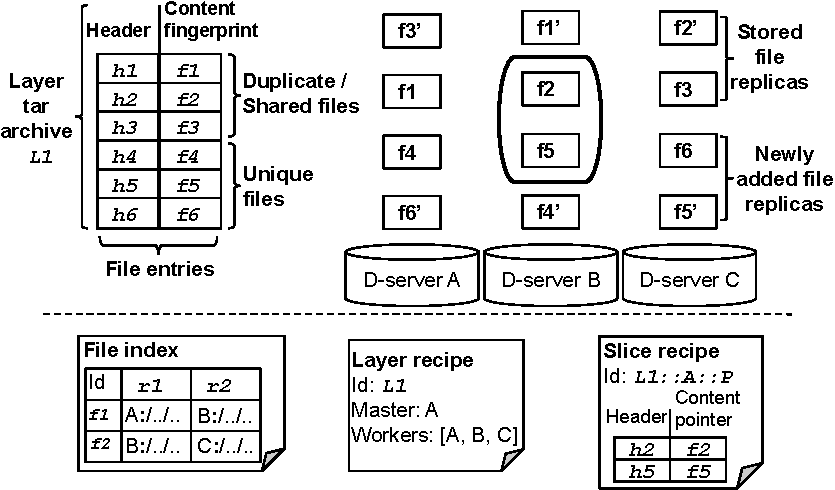
\includegraphics[width=\columnwidth]{graphs/replication.pdf}
	\caption{Layer dedup, replication, and partitioning.}
	\label{fig:replication-partition}
\end{figure}

%\begin{algorithm}
\scriptsize 
	\caption{Layer deduplication and partitioning}
	\label{alg:dedup-partition}
	\KwIn{\\	
			$FileIndex$: File index. \\
	}

	\KwOut{\\
			$LayerRecipe$: Layer recipe for layer $L$.\\
			$SliceRecipes$: Slice recipes for layer $L$' slices.\\
	}

	archive $\leftarrow$ \texttt{Decompress} layer $L$ \\

	\ForEach{header, content in archive} 
	{ 
		Id $\leftarrow$ \texttt{Hash} content \\
		%destHeader $\leftarrow$ header \\
		\eIf{ Id in FileIndex}{
			host  $\leftarrow$ $FileIndex$[Id].host \\
			src $\leftarrow$ $FileIndex$[Id].header \\
			{\tiny\texttt{/* SliceRecipe is identified by `layerid::host'}}
			SliceRecipe[$L::host$] $\leftarrow$  \texttt{Add} (header, src) \\
			{\tiny\texttt{/* Skip redundant file.  }}\\
		}{
			{\tiny\texttt{/* create file with content in file store.  }}\\
			file $\leftarrow$ \texttt{Create and write} content \\
			src $\leftarrow$ \texttt{Stat} file \\
			entries $\leftarrow$ (header, src)  \\
		}
	}
	
	\Do{entries}{
		{\tiny\texttt{/* get file entry with maximum file size. }}\\
		maxFile $\leftarrow$ \texttt{Max} entries \\
		{\tiny\texttt{/* get smallest slice. }}\\
		minSlice $\leftarrow$ \texttt{Min} SliceRecipes \\
		{\tiny\texttt{/* assign biggest file to smallest slice. }}\\
		minSlice $\leftarrow$ \texttt{Add} maxFile \\
		{\tiny\texttt{/* Set maxFile to FileIndex}}\\
		{\tiny\texttt{/* Remove maxFile from entries. }}\\
	}
	{\tiny\texttt{/* Send slices.}}\\
	{\tiny\texttt{/* Set SliceRecipes.}}\\
	{\tiny\texttt{/* Include all slices' hosts to workers.}}\\
	{\tiny\texttt{/* Select biggest slice' host as master.}}\\
	{\tiny\texttt{/* Set LayerRecipe.}}\\
	
	
		
\end{algorithm}




%<<<<<<< HEAD
%Then, the process sends slices to the corresponding registries.
Slice is identified by a simple combination of the layer id and its host address 
with the associated backup level,
denoted as $layerid::host::backuplevel$. % as shown in Algorithm~\ref{alg:dedup-partition}.
As shown in Figure~\ref{fig:replication-partition},
the primary slice stored on \emph{A} is denoted as \emph{L::}\emph{A::}\texttt{P}
while the rest backup slice is denoted as \emph{L::}\emph{A::}\texttt{B2}.
After unique file replication and layer partitioning, 
\sysname will add slice recipes 
to metadata database as shown in Figure~\ref{fig:dedup-partition}.
A slice recipe represents a layer slice and
is used to construct a \emph{partial layer archive}.
% 
%
As mentioned earlier, 
\sysname records every file header in a layer archive.
During layer partitioning,
%calculates the file id by hashing the file content.
%the file index maps a \emph{file id} to its associated physical file that is stored in the file store.
%To address a physical file,
%each file id in the file index holds its 
%denoted by a combination of its 
%\emph{host address} and \textbf{file status} of the physical file which mainly contains file name, path, and size.
%As shown in Algorithm~\ref{alg:dedup-partition}, 
%If a file's file id already exists in file index, 
%this file will be added to its host's corresponding partition (i.e, slice). 
%Otherwise,
%
%The file index is updated accordingly.
\sysname
assigns every file header in layer archive to
the associate slice recipe 
along with a content pointer pointing to the corresponding physical file as shown in Figure~\ref{fig:dedup-partition}. 
%=======
%Algorithm~\ref{alg:dedup-partition} details layer deduplication and partitioning algorithm.
%After layer decompression, 
%each file entry in the layer archive % subil: what is the layer archive referring to?
% is represented as a \textbf{file header} and a \textbf{file content}.
%The file header contains the file name, path, size, mode, owner information, etc. % subil: should elaborate on structure of the header, how is it constructed?
%The file header is needed to rebuild the \emph{file header} % subil: how are the two file headers different?
%for 
%the associated file entry in the layer archive.
%
%%During layer deduplication process,
%\sysname records each file entry's file header and 
%calculates the file id by hashing the file content.
%As mentioned earlier, the file index maps a \emph{file id} to its associated physical file that is stored in the file store.
%To address a physical file,
%each file id in the file index holds its 
%%denoted by a combination of its 
%\emph{host address} and \textbf{file status} of the physical file which mainly contains file name, path, and size.
%As shown in Algorithm~\ref{alg:dedup-partition}, 
%if a file's id already exists in file index (i.e. it's present in a registry server), 
%this file will be added to its host's corresponding slice for that layer. 
%Otherwise,
%\sysname stores the file content as a physical file in the file store
%and retrieves the file status of the physical file.
%The file index is updated accordingly.
%
%The slice recipe is identified by a simple combination of the layer id and its host registry address,
%denoted as $layerid::host$ as shown in Algorithm~\ref{alg:dedup-partition}.
%A slice recipe represents a layer partition and
%is used to construct a partial layer,
%>>>>>>> ab86d0a4767bfcfcbb58baf9bd7b2e81e54d7e51
%which
%records each file entry' $header$ in the layer archive partition and 
%its corresponding physical file's status . 
%In this case, 
%each file is represented as a $header$ in the layer archive and
%its corresponding physical file's status $src$. 



Finally, 
\sysname creates a
layer recipe for \emph{L} and stores in database as shown in Figure~\ref{fig:dedup-partition}.
Layer recipe records all the D-servers that stores \emph{L}'s slices, denoted as \textbf{restoring workers}.
One worker is selected as \textbf{restoring master} responsible for gathering all slices and rebuilding \emph{L} (detailed in Section~\ref{sec:restore-desgin}).
%During layer deduplication process,
%After unpacking the layer archive, 
%
%Note that destHeader can be used to rebuild the \textbf{file header} for 
%associated file entry in the layer archive.
%
 %its host' slice
%to get identical files' server addresses.

As shown in Figure~\ref{fig:replication-partition},
layer \emph{L} is evenly partitioned among D-servers 
since its shared files and unique files are evenly distributed to D-servers. 
However,
due to the diversity of real layer dataset,
shared files are usually not evenly distributed for all layers. 
To evenly distribute and partition layer's containing files,
%
%To distribute the newly added unique files' primary replicas,
\sysname uses a \emph{greedy partition algorithm with shared file constrains} to 
distribute the newly added unique files in a way such that
each D-server stores relatively equal-sized slice for the layer:
\sysname first assigns the shared files that are already stored on D-servers into 
their corresponding slices. 
Next,
\sysname
assigns the biggest unique file to the smallest slices
til all the unique files are assigned.
%After layer partition,.
%All the primary slices' hosts are denoted as layer restoring \textbf{primary workers}. 
%Next, \sysname stores slice recipes in metadata database after successfully
%sending slices to their corresponding workers.
%\sysname selects the biggest slice' host as layer restoring \textbf{primary master}.
%Layer recipe records the primary workers and master information for layer restoring.
%After that, \sysname~distributes primary slices' corresponding backup slices.
%Their hosts are denoted as \textbf{backup workers}.
%Finally, \sysname stores layer recipe in metadata database.
%Layer recipe 

%Here, we use the metadata database as a distributed lock for file index.
%File index sets a file id to hold  only if the file id does not exists.

%it uses a weighted round robin algorithm to distribute newly added 
%unique files to the registry cluster. These servers that already contains this layer's identical files
%are assigned a lower weight. 
%This is to ensue that different servers maintain same amount of files that are needed to restoring equal sized 
%slices for this layer.
%Deduplication process also 
%updates the \emph{file index} with the newly added unique files' fingerprints and host addresses.   
%Then, it calculates the slice fingerprints and creates a slice recipe for each slice.
%Slice recipe contains partial of the layer tarball's directory tree structure, file fingerprints, file name along with file path in the tarball, and file metadata information 
%(such as permissions and creation date), which are needed for restoring a slice for the layer. 

%After that
%After removing the duplicate files,
%Then, it
%distributes the \emph{deduplicated slices} evenly to the registry cluster by using round-robin, and,
%In the end, deduplication process creates a layer recipe which contains its slices' fingerprints and 
%based on layer recipe, it updates image manifests.
%The layer's tarball and file duplicates are removed after deduplication.

\subsection{Layer restoring}
\label{sec:restore-desgin}
%\paragraph{Parallel slice restoring}
%\label{subsubsec:slice-restoring}



\begin{figure}[t]
	\centering
	\centering
	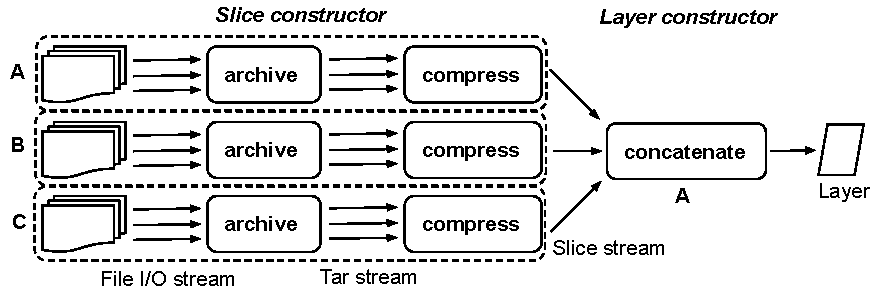
\includegraphics[width=\columnwidth]{graphs/sift-layer-construct-new.pdf}
	\caption{Parallel streaming layer construction.}
	\label{fig:construct}
\end{figure}



When a~\texttt{pull} layer request is received and its associated 
P-servers fail, 
\sysname will first search layer diskcache on D-servers.
If not found,
\sysname will rebuild the layer from file store according to its layer recipe. 
%the \dedupname~system 
%first prepares a directory structure for the slice, based on the slice recipe.
%Then, it copies the files into the directory tree.
%Next, it compresses the slice's directory tree into a slice tarball,
%and directly sends it back to the client.

\paragraph{Parallel layer construction}

When a~\texttt{pull} layer request is received, 
\sysname will update \emph{ULmap}. 
ULmap records user access status,
which maps a \textbf{user id} to its accessed layers with its corresponding access count,
where user id is defined as client request address.

Upon a \texttt{pull} layer request fails on P-servers,
\sysname initiates a layer restoring process on D-servers for it.
The process has two parts: slice constructor and layer constructor.
Figure~\ref{fig:restoring} shows an example of parallel layer restoring when a \texttt{pull} layer request failure happens.
First, 
layer constructor fetches the layer recipe from metadata database.
As shown in $L1$'s layer recipe, 
the primary restoring workers contains registry $A$, $B$, and $C$.
Since registry $A$ is the primary restoring master,
\emph{A} sends ``\texttt{Get primary slice}" requests to its peer workers: $B$ and $C$.
After a \texttt{Get primary slice} request is received, 
$B$ and $C$ start primary slice construction and return a primary slice back to $A$ respectively.
Meanwhile $A$ instructs local slice constructor to rebuild a primary slice for $L1$.
Slice constructor first gets its associate slice recipe (``$L1::P:A$") from metadata database 
keyed by a combination of  layer id, slice type (i.e., primary $P$ or backup $B \#$) and registry address.
Then, based on slice recipe,
slice constructor fetches files pointed by $Srcs$
and builds a slice archive.
After receiving all slices, layer constructor concatenates them into a compressed layer
and sends back the client. 

\paragraph{Streaming layer construction}
Figure~\ref{fig:construct} details the stateless streaming layer construction process.
First, slice constructor loads file in parallel from file store based on the slice recipe.
Each file is written to an archive buffer asynchronously.
Before writing file content to the archive buffer, slice constructor first builds and writes its
associated 
file header into the archive buffer according to the slice recipe. 
After archiving all the files in the slice,
the archive buffer will be divided into few chunks and compressed in parallel,
then concatenated into a single compressed slice stream.
Through network transfer, multiple slice streams will be concatenated into a single layer.
No intermediate file will be created or stored on disk. % subil: whoa!
\sysname uses a small file inmemory cache to reduce file I/Os. 
File cache uses Adaptive Replacement(ARC)~\cite{xxx}.

%headers according to $Dests$,
%after that it writes file contents into the archive
 
%Slice restoring process has four suboperations: 
%slice recipe lookup,
%slice file copying,
%slice compression, and
%slice network transfer. 
%To measure the overhead for each suboperation, 
%we implemented layer deduplication and parallel slice
%restoring on a 4-node registry cluster. 
%We first warmup the cluster by pushing 200 layers to the cluster
%and initiating layer deduplication process.
%The layers were randomly selected from our layer dataset detailed in xxx limited to 50MB.
%After finishing layer deduplication,
%we sent 400 \texttt{pull slice} requests to the cluster with 10 \texttt{pull slice} requests issued at a time.
%Figure~\ref{fig:slice-restoring-breakdown} shows the CDFs of the latencies for each suboperation.
%We see that across the four suboperations,
%the duration for slice compress is the shortest.
%Slice compression only took less than 0.001 s because a slice is a smaller unit. 
%The next shortest suboperation is network transfer since we pulled layer slice through Ethernet.
%90\% of slice recipe lookups took less than 0.1 s while 
%the highest slice recipe lookup duration almost reaches 0.8 s,
%which is caused by high concurrent lookup requests 
%%(note that we use redis to store metadata \NZ{use mongodb instead}).
%The most time consuming suboperation is slice file copying, which involves 
%copying all 
%the files that belong to the slice to their destination directory based on the slice recipe.
%Note that we implemented a thread pool on each registry server to read files in parallel
%and write data in RAMdisk to reduce disk IOs.
%40\%of slice file copying duration is greater than 1 s and 
%10\% of slice file copying duration is higher than 10 s.
%This is because bigger slices contains more files and requires more disk IOs.
%The overhead of slice copying can be largely mitigated for a large-scale registry cluster
%since the size of slice roughly equals to $S_{l}/N$, where $S_{l}$ denotes the layer size and $N$ is size of registry cluster.
%However, it could be a bottleneck for slice restoring on a small-scale registry cluster.
%%and slice file copying duration depends on slice size.
%
%%\begin{algorithm}
\scriptsize 
	\caption{File cache assisted slice restoring}
	\label{alg:file-cache}
	\KwIn{\\
		$\theta_{rsfc}$: Slice restoring latency threshold. \\
		$s$: Slice to be restored. \\
	}

	\SetKwFunction{Fsub}{Restore}
	\SetKwProg{Fn}{Function}{:}{}

	\Fn{\Fsub{s}}{
		%{\tiny\texttt{/* Otherwise, it's a repull layer miss   /}}\\
		\eIf{files in s are cached in file cache}
		{
			slice $\gets$ \texttt{RestoreSlice} \emph{s} \texttt{From} \emph{file cache + disk} 
		}
		{
			slice, $D_{rs}$ $\gets$ \texttt{RestoreSlice} \emph{s} \texttt{From} \emph{disk} \\
			\If{ $D_{rs} > \theta_{rsfc}$} 
			{ 
				\emph{file cache} $\gets$ \texttt{Cache} \texttt{Subsetof} \emph{s.files}
			}		
		}
	}

\end{algorithm}



%
%To reduce slice file copying overhead,
%\sysname~\filecachename~temporally cache a subset of unique files for bigger and popular slices that have a high slice restoring latency, ie., $D_{rs} > \theta_{rsfc}$, 
%where $D_{rs}$ is the slice restoring latency and $\theta_{rsfc}$ is the restoring latency threshold for 
%caching
%a subset of files from the slice to help improve its restoring performance as shown in Algorithm~\ref{alg:file-cache}.
%Upon a \texttt{pull slice} request for those slices, 
%\dedupname~ system fetches a subset of its containing files from \filecachename~and
%the remaining files from disk for slice restoring.
%
%To identify which slices have a high slice restoring latency,
%\dedupname~system monitors slice restoring performance and 
%maintains a restoring performance  profile for each slice that has been restored,
%% as shown in Figure~\ref{fig:xxx},
%which contains the latency breakdown of slice restoring
%% (,and a decompression latency updated by layer decompression process) 
%and its containing files' sizes.
%All the slice restoring performance profiles are also stored in distributed  databases,
% and addressed by slice digests. 
%To estimate the restoring latency for a slice $i$ that hasn't been restored, 
%\dedupname system~first lookups the slice restoring performance profiles by slice size,
% then selects a slice $x$ that is most similar in size to $i$,
% and estimates $i$'s restoring latency as: 
% $D_{rs}(i) \approx D_{rs}(x) + \Phi_{rs}(\Delta_{S})$,
% where $\Delta_{S}$ is the size different between two slices.
% $\Phi_{rs}(\Delta_{S})$ denotes a slice restoring latency function of slice size variation.
%  $\Phi_{rs}(\Delta_{S})$ is generated by using linear regression~\cite{xxx}.
% %$\varepsilon_{rs}$ is the standard error of restoring latency estimation for the layers similar in size.
%If the estimated slice restoring $D_{rs}(i) > \theta_{rs}$,
%then, \dedupname~lookups the slice restoring performance profiles by slice size,
%selects a slice $y$ that has a acceptable restoring latency and
%most similar in size to $i$.
%Next, \dedupname system~caches a subset of files $F$ for slice $i$, so that
%$D_{rs}(i) - \Phi_{rs}(\Sigma_{S}(F)) \approx D_{rs}(y)$,
%where $\Sigma_{S}(F)$ is the sum size of files in $F$.
%
%Note that \filecachename~size is limited so that \filecachename~only caches 
%subsets of files for big slices that belongs to popular layers.
%%that will be accessed later. 
%\cref{sec:cache-design} will describe how to determine popular layers based on user access patterns.
%Note that the slices for the same layer have similar sizes, restoring latencies, and popularity 
%because of unique file
%distribution. 
%Thus, once a layer is determined as popular layer, 
%\dedupname~will cache similar amount of files for its slices.
%Note that all the files in file cache are unique and can be shared for restoring different slices.
%
%For on-premise or private registry cluster, the network transfer speed is usually faster than remote cloud.
%Thus, slice compression is less important for medium to small size slices, 
%especially for the slices that have a high decompression latency, 
%i.e., $D_{stt} < \theta_{stt}$ and $D_{dc} > \theta_{dc}$, where $D_{stt}$ and $D_{dc}$ denote slice transfer duration
%and decompression duration respectively; 
%$\theta_{stt}$ and $\theta_{dc}$ denote thresholds for them respectively.
%Consequently, \dedupname system~only archives these slices without compressing them and directly sends
%these archival files back to the clients to eliminate clients' decompression latency.



